\documentclass{article}
\usepackage{listings}
\usepackage{graphicx}
\usepackage{xcolor}
\usepackage{geometry}

\geometry{a4paper, margin=1in}


% Farben für den Code-Block definieren
\lstset{
    basicstyle=\ttfamily\footnotesize,
    keywordstyle=\color{blue},
    commentstyle=\color{gray},
    stringstyle=\color{red},
    frame=single,
    breaklines=true,
    numbers=left,
    numberstyle=\tiny\color{gray},
}

\title{Erste Schritte in die Objekterkennung}
\author{}
\date{}

\begin{document}
\maketitle

\section*{Einführung }
Die Objekterkennung ist eine Kernkomponente vieler moderner Computer-Vision-Anwendungen. Sie ermöglicht es, Objekte in Bildern oder Videos zu identifizieren und ihre Positionen (Bounding Boxes) zu bestimmen. Dieses Verfahren basiert auf der Kombination von \textbf{maschinellem Lernen}, insbesondere \textbf{Deep Learning}, und Bildverarbeitungstechniken.

\section*{1. Grundprinzipien der Objekterkennung}
Die Objekterkennung umfasst zwei Hauptaufgaben:
\begin{itemize}
    \item \textbf{Klassifikation}: Bestimmung, um welches Objekt es sich handelt.
    \item \textbf{Lokalisierung}: Identifikation der Position des Objekts im Bild.
\end{itemize}

In modernen Systemen wie \textbf{YOLOv5} wird dies gleichzeitig durchgeführt. Die Architektur zerlegt die Aufgabe in die folgenden Schritte:
\begin{enumerate}
    \item \textbf{Feature Extraction}: Extraktion relevanter Merkmale aus dem Bild durch Convolutional Neural Networks (CNNs).
    \item \textbf{Region Proposals}: (Nur bei manchen Modellen) Erstellung von Vorschlägen für mögliche Positionen von Objekten.
    \item \textbf{Bounding Box Regression}: Präzise Bestimmung der Umrandungen der erkannten Objekte.
    \item \textbf{Klassifikation}: Zuordnung einer Objektklasse zu jeder Bounding Box.
\end{enumerate}

\textbf{YOLO} (You Only Look Once) verwendet ein End-to-End-System, bei dem alle diese Schritte in einem einzigen Durchgang durchgeführt werden. Das Modell unterteilt das Bild in ein Gitter und bestimmt in jedem Gitterfeld mögliche Objekte.

\section*{2. Verwendete Softwaresysteme}

\subsection*{a. YOLOv5}
\textbf{YOLOv5} ist eines der führenden Frameworks für Objekterkennung. Es ist bekannt für seine Geschwindigkeit und Genauigkeit. Die Pipeline basiert auf:
\begin{itemize}
    \item \textbf{PyTorch}: Eine Deep-Learning-Bibliothek für Training und Deployment des Modells.
    \item \textbf{Pretrained Models}: Vortrainierte Modelle wie COCO (Common Objects in Context) bieten eine breite Palette an erkennbaren Objekten.
    \item \textbf{NMS (Non-Maximum Suppression)}: Ein Algorithmus zur Auswahl der relevantesten Bounding Boxes bei überlappenden Vorhersagen.
\end{itemize}

\subsection*{b. NVIDIA Jetson Inference Toolkit}
Das Toolkit optimiert Modelle für den Einsatz auf NVIDIA Jetson Geräten. Es enthält:
\begin{itemize}
    \item Unterstützung für TensorRT: Eine NVIDIA-Technologie zur Beschleunigung von KI-Modellen.
    \item Werkzeuge zur Bildverarbeitung und Modellkonvertierung.
\end{itemize}

\subsection*{c. TensorRT}
\textbf{TensorRT} ist ein Framework für die Optimierung und Beschleunigung von Deep-Learning-Modellen auf NVIDIA-Hardware. Vorteile:
\begin{itemize}
    \item Reduzierte Latenz und beschleunigte Inferenz.
    \item Unterstützung für INT8-Quantisierung (Reduktion der Präzision zur Steigerung der Effizienz).
\end{itemize}

\subsection*{d. OpenCV}
\textbf{OpenCV} ist eine Open-Source-Bibliothek für Bildverarbeitung und Computer Vision:
\begin{itemize}
    \item Ermöglicht die Verarbeitung von Eingabebildern und Videos.
    \item Unterstützt die Visualisierung der Erkennungsergebnisse.
\end{itemize}

\section*{3. Schlüsseltechnologien im Hintergrund}

\subsection*{a. Deep Learning}
Die Objekterkennung basiert auf neuronalen Netzen, speziell Convolutional Neural Networks (CNNs). Diese Netze lernen Merkmale wie Kanten, Formen und Texturen und können daraus komplexe Muster erkennen.

\subsection*{b. GPU-Computing}
Da die Berechnungen für Deep-Learning-Modelle sehr aufwendig sind, werden GPUs (Graphics Processing Units) verwendet. NVIDIA Jetson Geräte und CUDA-Unterstützung sind wesentliche Bestandteile für die schnelle Verarbeitung.

\subsection*{c. Dataset und Training}
\begin{itemize}
    \item \textbf{COCO-Dataset}: Ein Standard-Datensatz, der häufig für das Training von Modellen wie YOLO verwendet wird.
    \item Modelle wie YOLOv5 nutzen Techniken wie Transfer Learning, um vortrainierte Netzwerke an spezifische Anwendungsfälle anzupassen.
\end{itemize}

\section*{4. Beispielhafter Workflow}
\begin{enumerate}
    \item \textbf{Installation}: YOLOv5 wird installiert und die erforderlichen Abhängigkeiten werden eingerichtet.
    \item \textbf{Modellinitialisierung}: Ein vortrainiertes YOLOv5-Modell wird geladen.
    \item \textbf{Datenverarbeitung}: Eingabebilder oder Video-Frames werden vorverarbeitet.
    \item \textbf{Inference}: Das Modell verarbeitet die Eingabe und liefert Bounding Boxes, Klassen und Konfidenzwerte zurück.
    \item \textbf{Visualisierung}: Die Ergebnisse werden mit OpenCV oder anderen Werkzeugen angezeigt.
\end{enumerate}

\section*{Zusammenfassung}
Die Kombination aus leistungsstarken Frameworks (\textbf{PyTorch}, \textbf{TensorRT}), Hardware (\textbf{Jetson}), und modernen Algorithmen (\textbf{YOLO}) macht die Objekterkennung effizient und vielseitig einsetzbar – von Überwachungskameras bis hin zu autonomen Fahrzeugen.


\clearpage
\section*{Software-Abhängigkeiten installieren}

\subsection*{1. Jetson-Inferenz-Toolkit}
NVIDIA bietet das \textbf{Jetson Inference}-Projekt an, das vortrainierte Modelle und Beispielanwendungen für Objekterkennung, Klassifikation und Segmentierung enthält.

\begin{lstlisting}[language=bash]
git clone --recursive https://github.com/dusty-nv/jetson-inference
# Falls der obige Befehl nicht funktioniert:
git clone --recursive --depth 1 https://github.com/dusty-nv/jetson-inference
\end{lstlisting}

Wechslen Sie ins Verzeichnis:
\begin{lstlisting}[language=bash]
cd jetson-inference
\end{lstlisting}

Überprüfen Sie den Status des Repositories:
\begin{lstlisting}[language=bash]
git status
\end{lstlisting}

\subsection*{2. Build-Prozess}
Erstellen Sie das Projektverzeichnis und bauen Sie das Projekt:
\begin{lstlisting}[language=bash]
cd jetson-inference
mkdir build
cd build
cmake ../
make -j$(nproc)
sudo make install
\end{lstlisting}

\subsection*{3. Python-Bibliotheken installieren}
Je nach Projekt können folgende Python-Bibliotheken installiert werden:

\begin{lstlisting}[language=bash]
sudo apt-get update
sudo apt-get install python3-pip
pip3 install numpy opencv-python matplotlib
pip3 install torch torchvision --extra-index-url https://download.pytorch.org/whl/cu118
\end{lstlisting}

\subsection*{4. YOLOv5/YOLONano verwenden}
Laden Sie YOLOv5 herunter und installieren Sie die Abhängigkeiten:
\begin{lstlisting}[language=bash]
git clone https://github.com/ultralytics/yolov5 
cd yolov5
pip3 install -r requirements.txt
python3 detect.py --source 0 
\end{lstlisting}
% python3 detect.py --source 0  Für Kamera-Input

Falls ein Fehler wie folgend auftritt: 
\textit{ValueError: numpy.dtype size changed, may indicate binary incompatibility. 
Expected 96 from C header, got 88 from PyObject}

Nutze diesen Befehl zur Behebung:
\begin{lstlisting}[language=bash]
pip3 install --upgrade --force-reinstall -r requirements.txt
\end{lstlisting}
Wiederholen Sie die vorherigen Schritte.

% \subsection*{5. Kamera-Setup und Videoaufnahme}
% Überprüfe, ob die Kamera funktioniert:
% \begin{lstlisting}[language=bash]
% gst-launch-1.0 nvarguscamerasrc ! nvoverlaysink
% \end{lstlisting}

% Für USB-Kameras:
% \begin{lstlisting}[language=bash]
% python3 detectnet-camera.py
% \end{lstlisting}

% \subsection*{6. Optimierung mit TensorRT}
% Beschleunige dein Modell mit \textbf{TensorRT}, um die Latenz zu reduzieren:
% \begin{lstlisting}[language=bash]
% sudo apt-get install tensorrt
% python3 trt_infer.py --engine model.trt
% \end{lstlisting}
\clearpage
\section{YOLOv5 startet}
die Kamera wird geöffnet und der Modell fängt an Objekte zu erkennen.
Dabei sieht der Terminal wie folgendes aus: 
\begin{figure}[h!]
    \centering
    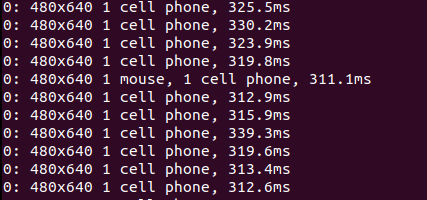
\includegraphics[width=0.8\textwidth]{Bilder/terminalErgebnisse.png}
\end{figure}

\section{Erkennungsbeispiele:}
Im folgenden sind ein paar Gegenstände, die mit YOLOv5 erkennt wurden.
\subsection{Handy}
Erkennung von Handy: 

\begin{center}
    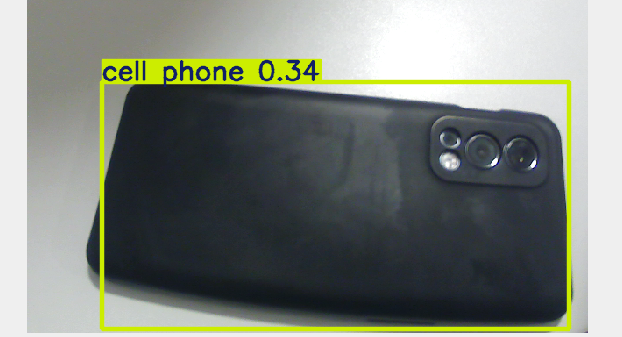
\includegraphics[width=0.8\textwidth]{Bilder/handyErkennung.png}
\end{center}

\subsection{Maus}
Erkeenung von Maus:

\begin{center}
    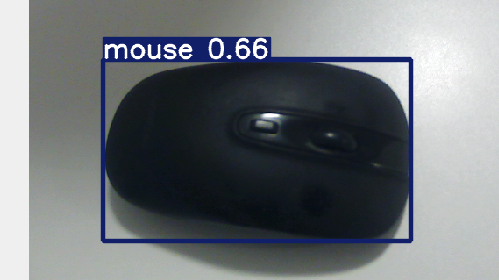
\includegraphics[width=0.8\textwidth]{Bilder/mausErkennung.png}
\end{center}

\subsection{Tastatur}
Erkennung von Tastatur: 

\begin{center}
    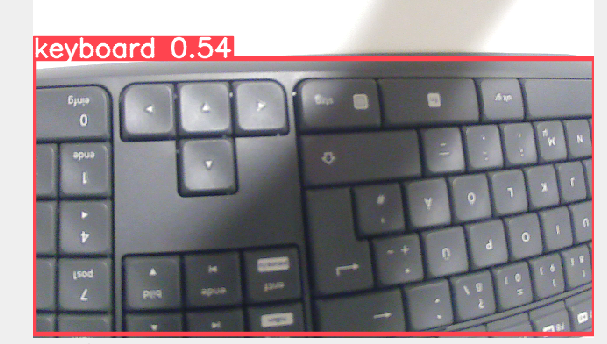
\includegraphics[width=0.8\textwidth]{Bilder/tastaturErkennung.png}
\end{center}
\end{document}
